%% -------------------------------------------------------------------
%% TikZ figure standalone: generate a pdf image
%% --------------------------------------------
\documentclass{standalone}

%% package needed
\usepackage{pgfplots}
\usepgfplotslibrary{groupplots}
\pgfplotsset{compat=newest}
\usetikzlibrary{positioning,arrows}
\usepgfplotslibrary{fillbetween}

%% Define the dimension
\newlength{\stabestimlwidth} \setlength{\stabestimlwidth}{2pt}
\newlength{\stabestimmwidth} \setlength{\stabestimmwidth}{6pt}
\newlength{\stabfreqwidth}   \setlength{\stabfreqwidth}  {10.5cm}
\newlength{\stabboundwidth}  \setlength{\stabboundwidth} {4pt}
\newlength{\modelwidth}      \setlength{\modelwidth}     {13.5cm}

%% begin the document which is only a TikZ picture
%% -----------------------------------------------
\begin{document}
%% -----------------------------------------------
%% begin the TikZ picture
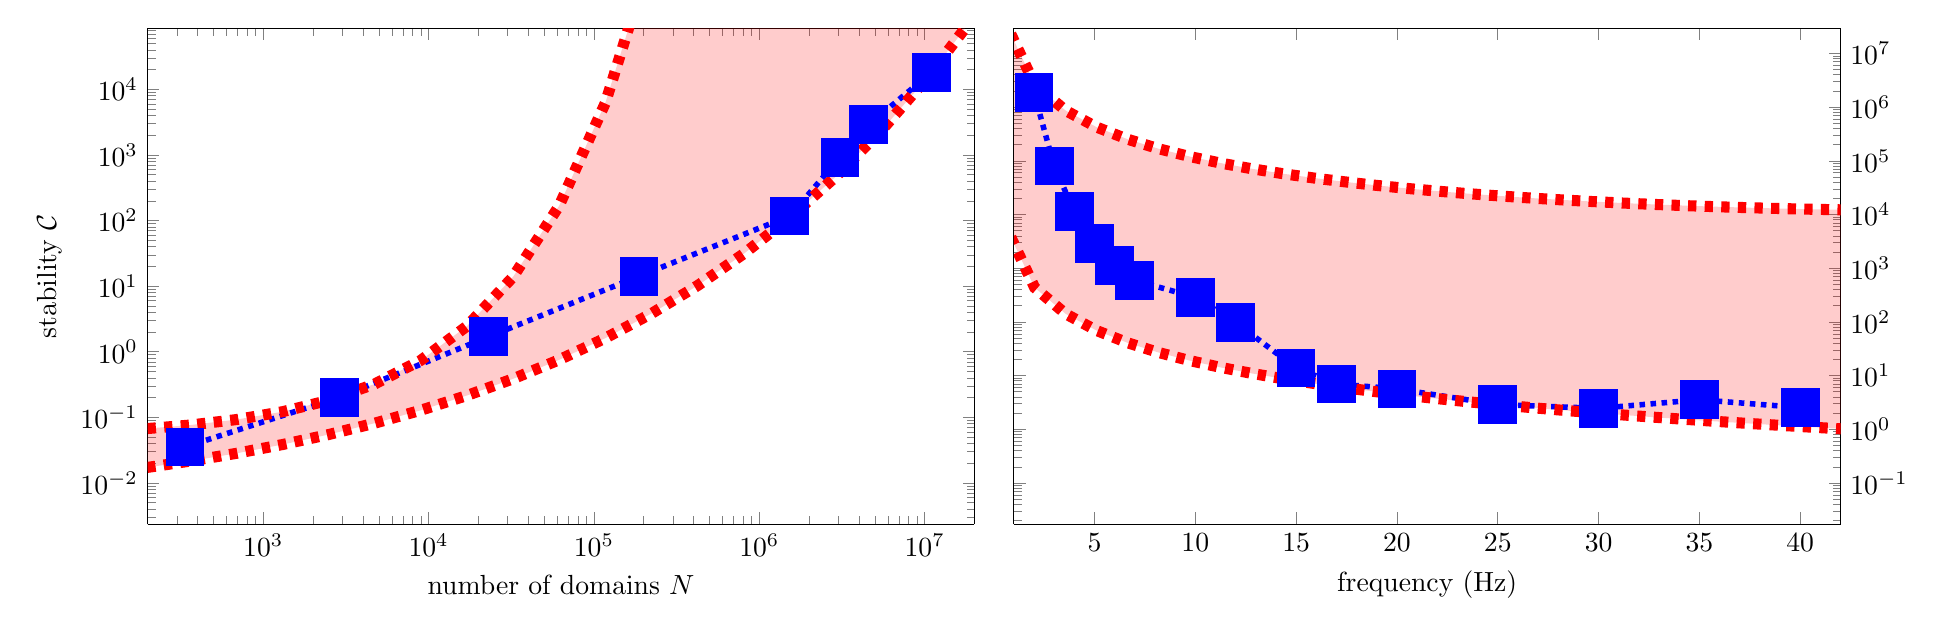
\begin{tikzpicture}
\begin{groupplot}[group style={group size=2 by 1,horizontal sep=.5cm,
                  group name=mygroupplot},ylabel={stability $\mathcal{C}$},
                  enlargelimits=false,xlabel={},
                  enlarge y limits=true,
                  clip=true,                     %% Necessary to make fill between works
                  set layers,cell picture=true,  %% Necessary to make fill between works
                  height=2\stabfreqwidth,width=1.2\stabfreqwidth]
%% Plot n°1 
%% -----------------------------------------------------------------------
   \nextgroupplot[height=.6\stabfreqwidth,width=\stabfreqwidth,
       scale only axis,separate axis lines,xminorticks=true,
       yminorticks=true, xmode=log,xlabel={number of domains $N$},
       ymode=log,xmin=200,xmax=2.e7,ymax=20000,ymin=1.e-2,
%%       clip mode=individual commented otherwize fillbetween explodes
       ]
     \pgfmathsetmacro{\omeg}{2.*5.*pi}
     \pgfmathsetmacro{\b}{1./1400}
     \pgfmathsetmacro{\kscaleu} {48.9390}%{11.7210}
     \pgfmathsetmacro{\kup}     {0.01489}%{0.03918}
     \pgfmathsetmacro{\kscalel} {11.7210}
     \pgfmathsetmacro{\klow}    {0.61010}
     
     \addplot [color=blue,dotted,mark=square*,mark options={solid},forget plot,
               line width=\stabestimlwidth,mark size=\stabestimmwidth]
       table[row sep=crcr]{%
          336   0.000000035275754E006  \\
         2880   0.000000201889140E006  \\
        23040   0.000001691598368E006  \\
       187492   0.000014179907670E006  \\
      1527168   0.000117216249820E006  \\
      3070818   0.000906557054637E006  \\
      4597248   0.002903951700096E006  \\
     11003850   0.018096826396902E006  \\
     };

     %% Upper Bound
     %% -----------
     \addplot[name path=up,color=red,dashed,forget plot,line width=\stabboundwidth,
              samples=20,domain=100:2.e7] 
               {\kscaleu / \omeg^2 * exp(\kup*(1+\omeg^2*\b^2)*x^(4./7.))};
     %% Lower Bound
     %% -----------
     \addplot[name path=low,color=red,dashed,forget plot,line width=\stabboundwidth,
              samples=20,domain=100:2.e7] 
              {\kscalel /(4.*\omeg^2) * exp(\klow*x^(1./5.))};
     \addplot[red,opacity=2.0e-01] fill between[of=up and low];


%% Plot n°2
%% ----------------------------------------------------------------------- 
   \nextgroupplot[height=.6\stabfreqwidth,width=\stabfreqwidth,
                  scale only axis,separate axis lines,xminorticks=true,
                  yminorticks=true,xmin=1, xmax=42,xlabel={frequency (Hz)},
                  ymode=log, ymin=0.1, ymax=5.e6,ylabel={},yticklabel pos=right]
     \pgfmathsetmacro{\Ndom}{4597248.}
     \pgfmathsetmacro{\b}{1./1400}
     \pgfmathsetmacro{\kup}{.0031}
     \pgfmathsetmacro{\klow}{.584}
     
     \addplot [color=blue,dotted,mark=square*,mark options={solid},forget plot,
               line width=\stabestimlwidth,mark size=\stabestimmwidth]
       table[row sep=crcr]{%
     2	1855716.87461442	\\
     3	80070.4361009	\\
     4	11298.166649348	\\
     5	2903.951700096	\\
     6	1120.555487093	\\
     7	590.08403191	\\
     %8	396.067979956	\\
     %9	320.232743003	\\
     10	287.337615622	\\
     12	98.035642042	\\
     15	13.780062743	\\
     17	6.985501224	\\
     20	5.651725837	\\
     25	2.883724849	\\
     30	2.453958595	\\
     35	3.546399113	\\
     40	2.536341391	\\
     };
     
     
     %% Upper Bound
     %% -----------
     \addplot[name path=up,color=red,dashed,forget plot,line width=\stabboundwidth,
              samples=30,domain=.5:45]
             {1./((2*pi*x)^2.) * exp(\kup*(1+(2*pi*x)^2*\b^2)*\Ndom^(4./7.))};
     %% Lower Bound
     %% -----------
     \addplot[name path=low,color=red,dashed,forget plot,line width=\stabboundwidth,
              samples=30,domain=.5:45]
              {1./(4.*(2*pi*x)^2) * exp(\klow*\Ndom^(1./5.))};
     \addplot[red,opacity=2.0e-01] fill between[of=low and up]; %soft clip={domain=-10:10}
   \end{groupplot}
\end{tikzpicture}
%% ----------------------
\end{document}
